
% Szkielet dla pracy inżynierskiej pisanej w języku polskim.

\documentclass[polish,bachelor,a4paper,oneside]{ppfcmthesis}

\usepackage[utf8]{inputenc}
\usepackage[OT4]{fontenc}
\usepackage{usecase}
\usepackage{float}
\usepackage[table]{xcolor}
\usepackage{mat}
\usepackage{verbatim}

% Authors of the thesis here. Separate them with \and
\author{%
   Adam Butkiewicz \album{98938} \and 
   Dominika Stempniewicz \album{89827} \and 
   Dawid Wengrzik \album{100191} \and
   Joanna Zakrzewska \album{99167}}
\title{LinkedInGrads: Otwarty System Monitorowania Karier Zawodowych Absolwentów}                   % Note how we protect the final title phrase from breaking
\ppsupervisor{dr hab.~inż.~Mikołaj Morzy} % Your supervisor comes here.
\ppyear{2014}                                         % Year of final submission (not graduation!)


\begin{document}

% Front matter starts here
\frontmatter\pagestyle{empty}%
\maketitle\cleardoublepage%

% Blank info page for "karta dyplomowa"
\thispagestyle{empty}\vspace*{\fill}%
\begin{center}\end{center}%
\vfill\cleardoublepage%

% Table of contents.
\pagenumbering{Roman}\pagestyle{ppfcmthesis}%
\tableofcontents* \cleardoublepage%

% Main content of your thesis starts here.
\mainmatter%
\chapter{Wprowadzenie}
\label{Chapter1}

\section{Opis problemu i koncepcja jego rozwiązania}
\label{Chapter11}

Zgodnie z rozporządzeniem Ministerstwa Nauki i Szkolnictwa Wyższego [1,2] każda uczelnia wyższa w Polsce jest zobowiązana do monitorowania karier swoich absolwentów, w celu pozyskania informacji o ich aktualnej sytuacji zawodowej. Oprócz spełnienia wymogów formalnych, systematyczne gromadzenie i analizowanie danych o zatrudnieniu absolwentów umożliwia uczelniom weryfikację jakości i efektywności kształcenia na poszczególnych wydziałach i kierunkach. Zebrane informacje stanowią cenną wskazówkę w ciągłym procesie doskonalenia oferty dydaktycznej uczelni, pomagając w dostosowywaniu kierunków studiów i programów kształcenia do potrzeb rynku pracy. Prowadzenie rzetelnych badań na temat losów zawodowych absolwentów i prezentowanie statystyk zatrudnienia jest również istotne z punktu widzenia wizerunku uczelni.

Ministerstwo Nauki i Szkolnictwa Wyższego nie narzuca uczelniom sposobu realizacji procesu monitorowania karier absolwentów. Większość uczelni wyższych, w tym Politechnika Poznańska, wywiązuje się z tego obowiązku za pomocą badania ankietowego. Opracowane ankiety są rozsyłane do absolwentów w formie elektronicznych lub drukowanych formularzy bądź przeprowadzane za pośrednictwem rozmów telefonicznych. Rozwiązania te są nie tylko kosztowne i czasochłonne, lecz charakteryzują się także niewielką efektywnością. Z szacunków Centrum Praktyk i Karier Politechniki Poznańskiej wynika,, że z możliwości dobrowolnego wypełnienia ankiety absolwenckiej korzysta poniżej 10% absolwentów.

W związku z wymienionymi wadami dotychczasowych metod zaproponowano stworzenie systemu informatycznego, w postaci aplikacji internetowej, który monitorowałby kariery zawodowe absolwentów wykorzystując dane udostępniane przez nich w serwisie LinkedIn. Serwis LinkedIn stanowi jedną z największych sieci zawodowych, łącząc ponad 250 mln. użytkowników w 200 krajach i terytoriach na całym świecie. Stworzony system powinien w założeniach zautomatyzować i uskutecznić proces monitorowania, pobierać dane o zatrudnieniu absolwentów z serwisu LinkedIn oraz prezentować je w formie raportów o z góry określonej strukturze. Należy przewidzieć również możliwość integracji z innymi serwisami mogącymi posłużyć jako źródło danych o sytuacji zawodowej absolwentów.

System został zrealizowany na Wydziale Informatyki Politechniki Poznańskiej w ramach zajęć Studia Rozwoju Oprogramowania. Wykonanie systemu zostało zlecone przez rzeczywistego klienta, w postaci przedstawicieli władz wydziału i uczelni. Prace były prowadzone według przyjętej metodyki i harmonogramu.

\section{Omówienie pracy}
\label{Chapter12}

Niniejsza praca opisuje otwarty system monitorowania karier zawodowych absolwentów LinkedInGrads (ang. LinkedInGrads: graduate career tracking system), zwany dalej Systemem, realizujący koncepcję przedstawioną w punkcie 1.1.  Praca stanowi dokumentację techniczną systemu, a także wyjaśnia idee stojące za poszczególnymi decyzjami projektowymi. Powinna być przydatna zarówno dla użytkowników końcowych systemu, jak i dla osób, które zamierzają go wdrożyć, utrzymywać bądź rozwijać. Jako praca dyplomowa inżynierska jest również skierowana do członków komisji egzaminacyjnej.

W rozdziale 2. przedstawiono aktorów, obiekty biznesowe oraz przypadki użycia występujące w systemie. W rozdziale 3. opisano wymagania funkcjonalne, a w rozdziale 4. wymagania pozafunkcjonalne, wraz z informacją, które z nich zostały zrealizowane. W rozdziale 5. omówiono ogólną architekturę systemu. Rozdział 6. zawiera szczegóły implementacji systemu oraz opis wykorzystanych koncepcji i technologii. W rozdziale 7. przedstawiono metody i narzędzia wspomagające zapewnienie jakości systemu. W rozdziale 8. opisano zebrane wnioski i doświadczenia. Rozdział 9. zawiera podsumowanie całości projektu oraz propozycje dalszego rozwoju systemu. W skład dokumentu wchodzi również bibliografia pracy oraz dodatki, obejmujące informacje uzupełniające, prezentację wyglądu aplikacji, instrukcję instalacji oraz scenariusze manualnych testów akceptacyjnych.
\chapter{Opis procesów biznesowych}
\label{Chapter2}

\section{Aktorzy}
\label{Chapter21}

Wymienienie aktorów zdefiniowanych dla systemu (np. jako wyliczenia).

\section{Obiekty biznesowe}
\label{Chapter22}

\subsection{Obiekt 1}

Opis obiektu pierwszego, jego zastosowania. Poniżej wymieniamy jego atrybuty (jeśli istnieją):

\begin{itemize}
\item Atrybut 1
\item Atrybut 2
\item ...
\end{itemize}

\subsection{Obiekt 2}

Ponownie opis, tym razem dla obiektu drugiego. Oczywiście, inne obiekty opisujemy tak samo:

\begin{itemize}
\item Atrybut 1
\item Atrybut 2
\item ...
\end{itemize}

\pagebreak
\section{Biznesowe przypadki użycia}
\label{Chapter23}

Poniżej przedstawiacie biznesowe przypadki użycia. Proponuję tutaj wykorzystać szablon, który również jest przerobionym szablonem LaTeXowym i dostosowanym do naszych potrzeb, specjalnie dla opisywania przypadków użycia.

\subsection{ID01: Nazwa przypadku użycia}

\ucsection{ID01: Nazwa przypadku użycia}{Aktor 1, Aktor 2}
{}{}
\ucactions{
\ucaction{1. Pierwszy punkt głównego scenariusza}
\ucaction{2. Drugi punkt głównego scenariusza}
\ucaction{3. Trzeci punkt głównego scenariusza}
}}
{\ucextensions{
\ucaction{3.A Opis sytuacji wyjątkowej 1}
\ucaction{3.A.1 Pierwszy krok sytuacji wyjątkowej 1}
\ucaction{3.B Opis sytuacji wyjątkowej 2}
\ucaction{3.B.1 Pierwszy krok sytuacji wyjątkowej 2}
\ucaction{3.B.2 Drugi krok sytuacji wyjątkowej 2}
}}
{}

\subsection{ID02: Przykład przypadku użycia bez wyjątków}

\ucsection{ID02: Przykład przypadku użycia bez wyjątków}{Aktor 1}
{}
{}{\ucactions{
\ucaction{1. Pierwszy punkt głównego scenariusza}
\ucaction{2. Drugi punkt głównego scenariusza}
\ucaction{3. Trzeci punkt głównego scenariusza}
}}
{}

\section{Opis procesów biznesowych z wykorzystaniem notacji graficznej}
\label{Chapter24}

Ten podrozdział jest opcjonalny (a może nawet można to przedstawić jako podsekcję poprzedniego podrozdziału). Tutaj możemy pochwalić się diagramem (np.~BPMN) dla naszych procesów biznesowych. Oczywiście, nie tylko w formie graficznej -- jeśli macie inną formę, to też się nadaje (o ile jest ona przyzwoita).
\chapter{Wymagania funkcjonalne}
\label{Chapter3}

Wymagania funkcjonalne (ang. functional requirements) określają co system powinien oferować użytkownikowi, to jest jakie operacje można na nim wykonać. Ważne jest, by utrzymać kompletny zbiór poprawnie zdefiniowanych wymagań, pomaga to w zrozumieniu w jaki sposób powinien działać system, nawet dla osób które nie mają wiedzy technicznej oraz pomaga podczas jego projektowania.

Niniejszy rozdział przedstawia wymagania funkcjonalne za pomocą dwóch najpopularniejszych sposobów ich opisu, są to: przypadki użycia (ang. use cases)  oraz opowieści użytkownika (ang. user stories). Pierwsza z metod polega na określeniu listy kroków. Reprezentuje ona interakcję między aktorem a systemem. Wykonanie kroków skutkuje osiągnięciem celu, który ma zapewnić system. Druga metoda - Opowieści użytkownika przedstawia w kilku zdaniach potrzebę użytkownika, którą ma realizować system. 

\begin{figure}[th] 
\centering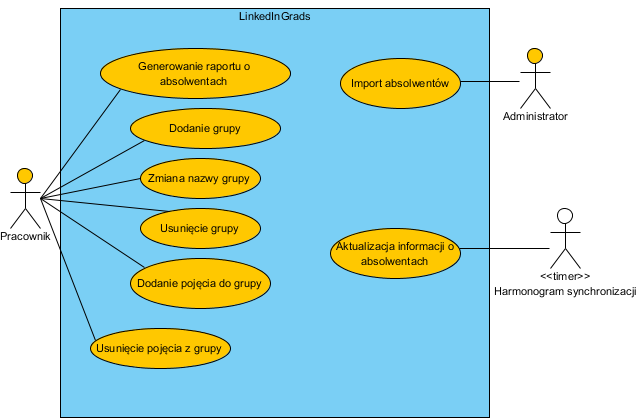
\includegraphics[width=15cm]{figures/image1}
\caption{Diagram przypadków użycia}\label{rys:use-case-diagram}
\end{figure}

\subsection{Generowanie raportu o absolwentach}

\ucsection{UC1: Generowanie raportu o absolwentach}{Pracownik dziekanatu, System}
{}
{}{\ucactions{
\ucaction{1. Pracownik wybiera opcję generowania raportu.}
\ucaction{2. System prezentuje typy raportów do wyboru.}
\ucaction{3. Pracownik wybiera typ raportu.}
\ucaction{4. System prezentuje rok ukończenia studiów do wyboru.}
\ucaction{5. Pracownik wybiera rok ukończenia studiów.}
\ucaction{6. Pracownik inicjuje generowanie raportu.}
\ucaction{7. System prosi o wybranie ścieżki zapisu raportu.}
\ucaction{8. Pracownik wybiera ścieżkę zapisu.}
}}
{}

\subsection{Dodanie grupy}

\ucsection{UC2: Dodanie grupy}{Pracownik dziekanatu, System}
{}
{}{\ucactions{
\ucaction{1. Pracownik wybiera opcję dodania grupy.}
\ucaction{2. System prosi o podanie nazwy grupy.}
\ucaction{3. Pracownik podaje nazwę grupy.}
\ucaction{4. System informuje o pomyślnym dodaniu grupy.}
}}
{\ucextensions{
\ucaction{3.A. Grupa o podanej nazwie już istnieje.}
\ucaction{3.A.1. System informuje o błędzie.}
\ucaction{3.A.2. Powrót do kroku 3.}
}}
{}

\subsection{Zmiana nazwy grupy}

\ucsection{UC3: Zmiana nazwy grupy}{Pracownik dziekanatu, System}
{}
{}{\ucactions{
\ucaction{1. Pracownik wybiera opcję zmiany nazwy grupy.}
\ucaction{2. System prezentuje listę istniejących grup.}
\ucaction{3. Pracownik wybiera grupę.}
\ucaction{4. System prosi o podanie nowej nazwy grupy.}
\ucaction{5. Pracownik podaje nową nazwę grupy.}
\ucaction{6. System informuje o pomyślnej zmianie nazwy grupy.}
}}
{\ucextensions{
\ucaction{5.A. Grupa o podanej nazwie już istnieje.}
\ucaction{5.A.1. System informuje o błędzie.}
\ucaction{5.A.2. Powrót do kroku 3.}
}}
{}

\subsection{Usunięcie grupy}

\ucsection{UC4: Usunięcie grupy}{Pracownik dziekanatu, System}
{}
{}{\ucactions{
\ucaction{1. Pracownik wybiera opcję usunięcia grupy.}
\ucaction{2. System prezentuje listę istniejących grup.}
\ucaction{3. Pracownik wybiera grupę do usunięcia.}
\ucaction{4. System informuje o pomyślnym usunięciu grupy.}
}}
{}

\subsection{Dodanie pojęcia do grupy}

\ucsection{UC5: Dodanie pojęcia do grupy}{Pracownik dziekanatu, System}
{}
{}{\ucactions{
\ucaction{1. Pracownik wybiera opcję grupowania pojęć.}
\ucaction{2. System prezentuje listę istniejących grup.}
\ucaction{3. Pracownik wybiera grupę.}
\ucaction{4. System prezentuje listę pojęć niezgrupowanych.}
\ucaction{5. Pracownik wybiera pojęcie do dodania.}
\ucaction{6. System informuje o pomyślnym dodaniu pojęcia do grupy.}
}}
{\ucextensions{
\ucaction{3.A. Grupa została w międzyczasie usunięta.}
\ucaction{3.A.1. System informuje o błędzie.}
\ucaction{3.A.2. Powrót do kroku 2.}
\ucaction{5.A. Grupa została w międzyczasie usunięta.}
\ucaction{5.A.1. System informuje o błędzie.}
\ucaction{5.A.2. Powrót do kroku 2.}
}}
{}

\subsection{Usunięcie pojęcia z grupy}

\ucsection{UC6: Usunięcie pojęcia z grupy}{Pracownik dziekanatu, System}
{}
{}{\ucactions{
\ucaction{1. Pracownik wybiera opcję grupowania pojęć.}
\ucaction{2. System prezentuje listę istniejących grup.}
\ucaction{3. Pracownik wybiera grupę.}
\ucaction{4. System prezentuje listę pojęć przypisanych do grupy.}
\ucaction{5. Pracownik wybiera pojęcie do usunięcia.}
\ucaction{6. System informuje o pomyślnym usunięciu pojęcia z grupy.}
}}
{\ucextensions{
\ucaction{3.A. Grupa została w międzyczasie usunięta.}
\ucaction{3.A.1. System informuje o błędzie.}
\ucaction{3.A.2. Powrót do kroku 2.}
}}
{}

\subsection{Aktualizacja informacji o absolwentach}

	\begin{tabular}{| p{.9\textwidth} |}
		\hline
		\textbf{Opowieść użytkownika:} US1 \\
		\hline
		\textbf{Opis:} Przebieg aktualizacji informacji o absolwentach. Odbywa się automatycznie, w tle działającego systemu. \\
		\hline
		\textbf{Treść:} Jako Pracownik chcę aby System, co ustalony czas pobierał informacje o absolwentach z portalu LinkedIn, a
następnie aktualizował swoją bazę danych. \\
		\hline  
	\end{tabular}
	
\subsection{Import absolwentów}

\ucsection{UC7: Import absolwentów}{Administrator, System}
{}
{}{\ucactions{
\ucaction{1. Pracownik wywołuje skrypt importu absolwentów.}
\ucaction{2. System prezentuje listę dodanych absolwentów.}
}}
{\ucextensions{
\ucaction{1.A. Niepoprawne dane wejściowe.}
\ucaction{1.A.1. System przerywa import i informuje o błędzie.}
\ucaction{1.A.2. Powrót do 1.}
}}
{}	

\subsection{Grupowanie pojęć}

	\begin{tabular}{| p{.9\textwidth} |}
		\hline
		\textbf{Opowieść użytkownika:} US2 \\
		\hline
		\textbf{Opis:} Generowanie raportu z użyciem mechanizmu grupowania pojęć. \\
		\hline
		\textbf{Treść:} Jako Pracownik chcę aby pojęcia (umiejętności, stanowiska, organizacje) w wygenerowanym raporcie były
pogrupowane (np. za pomocą metody LDA) w bardziej ogólne zbiory. 
 \\
		\hline  
	\end{tabular}
\chapter{Wymagania pozafunkcjonalne}
\label{Chapter4}

Wymagania pozafunkcjonalne (ang. non-functional requirements) określają jakość sposobu realizacji funkcji przez system. Mimo, że wymagania funkcjonalne uda się spełnić, to nie zawsze realizacja celu jest w stanie usatysfakcjonować odbiorcę systemu. Dobrze sprecyzowane wymagania pozafunkcjonalne pozwalają na uniknięcie niskiej użyteczności systemu oraz mogą mieć wpływ na sam sposób realizacji projektu. Stworzenie i weryfikacja tych wymagań jest ważna zarówno dla zlecającego projekt jak i wykonawcy projektu, gdyż doprecyzowują one użyteczność korzystania z systemu, co pozwala na uniknięcie sporów podczas odbioru projektu, w przypadku niskiej jego jakości. Jakość uzyskanego systemu ma również wpływ na jego późniejsze utrzymanie po stronie klienta, stąd tak ważne rozsądne opisanie wymagań pozafunkcjonalnych, które nie zawsze potrafią być oczywiste dla użytkowników końcowych.

\section{Standard ISO/IEC FDIS 25010}

Model jakości oprogramowania standardu ISO/IEC FDIS 25010 [3] wyróżnia następujące charakterystyki i podcharakterystyki jakości oprogramowania:

\begin{itemize}
\item Funkcjonalne dopasowanie (ang. Functional suitability)
	\begin{itemize}
	\item Funkcjonalna kompletnosc (ang. Functional completeness)
	\item Funkcjonalna odpowiedniość (ang. Functional correctness)
	\item Funkcjonalna poprawność (ang. Functional appropriateness)
	\end{itemize}
\item Wydajność (ang. Performance efficiency)
	\begin{itemize}
	\item Charakterystyka czasowa (ang. Time behaviour)
	\item Zużycie zasobów (ang. Resource utilization)
	\item Oczekiwana wydajność (ang. Capacity)
	\end{itemize}
\item Kompatybilność (ang. Compatibility)
	\begin{itemize}
	\item Współistnienie (ang. Co-existence)
	\item Interoperacyjność (ang. Interoperability)
	\end{itemize}
\item Użyteczność (ang. Usability)
	\begin{itemize}
	\item Rozpoznawalność zastosowania (ang. Appropriateness recognizability)
	\item Łatwość nauczenia się (ang. Learnability)
	\item Łatwość operowania (ang. Operability)
	\item Ochrona użytkownika przed błędami (ang. User error protection)
	\item Estetyka interfejsu użytkownika (ang. User interface aesthetics)
	\item Dostępność personalna (ang. Accessibility)
	\end{itemize}
\item Niezawodność (ang. Reliability)
	\begin{itemize}
	\item Dojrzałość (ang. Maturity)
	\item Tolerancja uszkodzeń (ang. Availability)
	\item Odporność na wady (ang. Fault tolerance)
	\item Odtwarzalność (ang. Recoverability)
	\end{itemize}
\item Bezpieczeństwo (ang. Security)
	\begin{itemize}
	\item Poufność (ang. Confidentiality)
	\item Integralność (ang. Integrity)
	\item Niezaprzeczalność (ang. Non-repudiation)
	\item Identyfikowalność (ang. Accountability)
	\item Autentyczność (ang. Authenticity)
	\end{itemize}
\item Łatwość utrzymania (ang. Maintainability)
	\begin{itemize}
	\item Modułowość (ang. Modularity)
	\item Łatwość ponownego wykorzystania (ang. Reusability)
	\item Łatwość analizy (ang. Analysability)
	\item Łatwość zmiany (ang. Modifiability)
	\item Łatwość testowania (ang. Testability)
	\end{itemize}
\item Przenośność (ang. Portability)
	\begin{itemize}
	\item Łatwość adaptacji (ang. Adaptability)
	\item Łatwość instalacji (ang. Installability)
	\item Łatwość zamiany (ang. Replaceability)
	\end{itemize}
\end{itemize}

Wymienione podcharakterystyki posłużyły jako kategorie wymagań pozafunkcjonalnych w projekcie. Ze względu na specyfikę systemu - aplikacji internetowej niektóre kategorie tego standardu nie zostały wykorzystane podczas prac nad wymaganiami pozafunkcjonalnymi.

\section{Wymagania pozafunkcjonalne i ich weryfikacja}

W kolejnych tablicach przedstawiono wymagania pozafunkcjonalne systemu LinkedInGrads, określonych przy pomocy standardu ISO/IEC FDIS 25010. Priorytet wymagań określono za pomocą notacji:

\begin{itemize}
\item Would - System może spełniać dane wymaganie,
\item Should - System powinien spełniać dane wymaganie,
\item Must - System musi spełniać dane wymaganie.
Dodatkowo określono złożoność każdego z wymagań wykorzystując następującą notację:
\item Low - Niski stopień złożoności wymagania pozafunkcjonalnego,
\item Medium - Średni stopień złożoności wymagania pozafunkcjonalnego,
\item High - Wysoki stopień złożoności wymagania pozafunkcjonalnego.
Metryki te pozwalały podczas prac nad projektem na realizację najważniejszych wymagań, uwzględniając ich złożoność czasową skonfrontowaną z dostępnym czasem na realizację projektu. Ostatnia kolumna tabeli określa czy w projekcie LinkedInGrads udało się spełnić dane wymaganie pozafunkcjonalne.
\end{itemize}

\subsection{Funkcjonalne dopasowanie: Funkcjonalna kompletność}

\begin{table}[H]
\centering
\begin{tabular}{ | p{8cm} | c | c | c | }
\hline
\textbf{Wymaganie} & \textbf{Priorytet} & \textbf{Złożoność} & \textbf{Realizacja} \\ \hline
Współpraca z przeglądarką Firefox (dla dwóch najnowszych wersji). & Must & Low & Zrealizowano \\ \hline
\end{tabular}
\caption{Funkcjonalne dopasowanie: Funkcjonalna kompletność}\label{tab:reqs}
\end{table}

System był tworzony wykorzystując do testów najnowszą wersję przeglądarki Mozilla Firefox, oraz dodatkowo Google Chrome. Zapewniło to kompatybilność systemu z tymi przeglądarkami, a funkcje użyte wewnątrz systemu nie wykraczają poza zakres możliwości poprzednich kilku wersji tych przeglądarek.

\subsection{Wydajność: Charakterystyka Czasowa}

\begin{table}[H]
\centering
\begin{tabular}{ | p{8cm} | c | c | c | }
\hline
\textbf{Wymaganie} & \textbf{Priorytet} & \textbf{Złożoność} & \textbf{Realizacja} \\ \hline
Dla 20000 absolwentów aktualizacja danych
z LinkedIn nie powinna trwać dłużej niż
tydzień. & Must & Medium & Zrealizowano \\ \hline
System powinien estymować czas
aktualizacji danych. & Would & High & Pominęto \\ \hline
Generowanie raportu nie może trwać dłużej
niż 10 sekund - w przeciwnym wypadku
informacja o czasie. & Should & Medium & Zrealizowno \\ \hline
\end{tabular}
\caption{Wydajność: Charakterystyka Czasowa}\label{tab:reqs}
\end{table}

Wymagania tej kategorii udało się spełnić, a dzięki aktualizacji danych w tle, estymacja czasu zakończenia aktualizacji okazała się zbędna w finalnej wersji produktu, co również spowodowało niski czas generowania raportu.

\subsection{Kompatybilność: Współistnienie}

\begin{table}[H]
\centering
\begin{tabular}{ | p{8cm} | c | c | c | }
\hline
\textbf{Wymaganie} & \textbf{Priorytet} & \textbf{Złożoność} & \textbf{Realizacja} \\ \hline
Na jednym serwerze może być
uruchomionych wiele instancji aplikacji. & Would & Medium & Zrealizowano \\ \hline
\end{tabular}
\caption{Kompatybilność: Współistnienie}\label{tab:reqs}
\end{table}

Wymaganie to zostało zrealizowane na poziomie architektury poprzez wykorzystanie aplikacji internetowej uruchamianej w środowisku serwera WWW.

\subsection{Kompatybilność: Interoperacyjność}

\begin{table}[H]
\centering
\begin{tabular}{ | p{8cm} | c | c | c | }
\hline
\textbf{Wymaganie} & \textbf{Priorytet} & \textbf{Złożoność} & \textbf{Realizacja} \\ \hline
System ma udostępniać dane absolwenta w
trybie odczytu w formacie JSON przez webservice.
 & Should & High & Pominięto \\ \hline
System ma generować raporty w formacie
CSV.
 & Should & Low & Pominęto \\ \hline
System ma generować raporty w formacie
XLS.
 & Must & Low & Zrealizowano \\ \hline
\end{tabular}
\caption{Kompatybilność: Interoperacyjność}\label{tab:reqs}
\end{table}

Ze względu na duży narzut czasowy wymagań pozafunkcjonalnych z tej kategorii udało się zrealizować tylko generowanie raportu w formacie XLS. Pominięte wymagania funkcjonalne nie były kluczowe dla systemu, co spowodowało, że ich realizacja nie została przydzielona do żadnego ze sprintów.

\subsection{Użyteczność: Łatwość nauczenia się}

\begin{table}[H]
\centering
\begin{tabular}{ | p{8cm} | c | c | c | }
\hline
\textbf{Wymaganie} & \textbf{Priorytet} & \textbf{Złożoność} & \textbf{Realizacja} \\ \hline
Interfejs użytkownika powinien być skonsultowany ze wszystkimi potencjalnymi użytkownikami.
 & Must & Low & Zrealizowano \\ \hline
Instrukcja użytkownika powinna być zorientowana na cele poszczególnych aktorów.
 & Must & Low & Zrealizowano \\ \hline
\end{tabular}
\caption{Użyteczność: Łatwość nauczenia się}\label{tab:reqs}
\end{table}

Zespół był wysoce zorientowany na potrzeby użytkownika końcowego, co już w samej fazie projektowania interfejsów użytkownika zapewniło wysoką jakość systemu. Po skonsultowaniu z użytkownikami, wdrożono udoskonalenia co pozwoliło na zrealizowanie wymagania pozafunkcjonalnego.

\subsection{Użyteczność: Ochrona użytkownika przed błędami}

\begin{table}[H]
\centering
\begin{tabular}{ | p{8cm} | c | c | p{2cm} | }
\hline
\textbf{Wymaganie} & \textbf{Priorytet} & \textbf{Złożoność} & \textbf{Realizacja} \\ \hline
System musi być przygotowany na rozszerzenie list atrybutów.
 & Must & Low & Zrealizowano \\ \hline
System powinien logować błedy (wyjątki) do logu systemowego.
 & Must & Low & Zrealizowano \\ \hline
 System powinien informować o błędnej konfiguracji natychmiast po jej wprowadzeniu. & Would & Medium & Pominięto \\ \hline
 System ma potwierdzać powiązanie/odwiązanie użytkownika. & Would & Low & Pominięto \\ \hline
 System powinien zapewnić kontrolę nieprzewidzianych wyjątków. & Must & Low & Zrealizowano częściowo. \\ \hline
 Po wykonaniu importu danych system informuje ilu absolwentów zaimportowano, a ile jest konfliktów. & Must & Low & Pominięto \\ \hline
\end{tabular}
\caption{Użyteczność: Ochrona użytkownika przed błędami}\label{tab:reqs}
\end{table}

System został przygotowany mając od początku na uwadze możliwość rozszerzenia go o  dodatkowe dane jak i dodatkowe źródła danych, co zapewniło realizację pierwszego z wymagań. Wszystkie błędy które pojawią się w aplikacji automatycznie zapisywane są do logów, co częściowo realizuje również wymaganie dotyczące kontroli nieprzewidzianych wyjątków, które zostają w momencie wystąpienia ukryte przed użytkownikiem końcowym. Podczas prac nad systemem zrezygnowano z możliwości konfiguracji parametrów jego pracy, ze względu na brak zasadności jakichkolwiek zmian. Wymaganie to powstało mając na uwadze możliwe ograniczenia narzucone na system pochodzące z zewnętrznych źródeł danych. Również w trakcie prac zrezygnowano z automatycznego wyszukiwania użytkowników wewnątrz sieci społecznościowej LinkedIn i wiązania znalezionych kont z danymi osób dostarczonymi z dziekanatu. Wyeliminowało to potrzebę potwierdzania powiązania/odwiązania użytkownika, gdyż dane te wprowadzane są manualnie przez użytkownika. Ostatnie z wymagań nie zostało zrealizowane ze względu na dołączenie go do wymagań pozafunkcjonalnych w późnej fazie projektu i nie uwzględnienie jego realizacji w żadnym ze sprintów.

\subsection{Użyteczność: Estetyka interfejsu użytkownika}

\begin{table}[H]
\centering
\begin{tabular}{ | p{8cm} | c | c | c | }
\hline
\textbf{Wymaganie} & \textbf{Priorytet} & \textbf{Złożoność} & \textbf{Realizacja} \\ \hline
Interfejs powinien zawierać logo Politechniki Poznańskiej oraz opis przeznaczenia systemu.
 & Must & Low & Zrealizowano \\ \hline
\end{tabular}
\caption{Użyteczność: Estetyka interfejsu użytkownika}\label{tab:reqs}
\end{table}

\subsection{Użyteczność: Dostępność personalna}

\begin{table}[H]
\centering
\begin{tabular}{ | p{8cm} | c | c | c | }
\hline
\textbf{Wymaganie} & \textbf{Priorytet} & \textbf{Złożoność} & \textbf{Realizacja} \\ \hline
System dostępny tylko w jednej wersji językowej - Polskiej
 & Must & Low & Zrealizowano \\ \hline
\end{tabular}
\caption{Użyteczność: Dostępność personalna}\label{tab:reqs}
\end{table}

\subsection{Niezawodność: Tolerancja uszkodzeń}

\begin{table}[H]
\centering
\begin{tabular}{ | p{8cm} | c | c | c | }
\hline
\textbf{Wymaganie} & \textbf{Priorytet} & \textbf{Złożoność} & \textbf{Realizacja} \\ \hline
Przerwy serwisowe możliwe są w godzinach 18-6 lub po wcześniejszym ustaleniu.
 & Should & Low & Pominięto \\ \hline
 Niekontrolowana awaria może trwać maksymalnie 2 dni. & Should & Low & Pominięto \\ \hline
\end{tabular}
\caption{Niezawodność: Tolerancja uszkodzeń}\label{tab:reqs}
\end{table}

Wymagania należące do tej kategorii nie zostały zrealizowane. Wynika to z faktu, że dotyczą one utrzymania systemu po jego wdrożeniu, więc weryfikacja tych wymagań była niemożliwa do przeprowadzenia.	

\subsection{Niezawodność: Odporność na wady}

\begin{table}[H]
\centering
\begin{tabular}{ | p{8cm} | c | c | c | }
\hline
\textbf{Wymaganie} & \textbf{Priorytet} & \textbf{Złożoność} & \textbf{Realizacja} \\ \hline
System należy poddać analizie z wykorzystaniem metody ATAM.
 & Must & Low & Zrealizowano \\ \hline
Wszystkie funkcje głównego scenariusza powinny być możliwe do przetestowania w sposób automatyczny.
 & Should & Low & Zrealizowano \\ \hline
W przypadku problemów z połączeniem, proces aktualizacji danych powinien być wznawiany (od stanu w którym nastąpiło przerwanie). & Would & Low & Zrealizowano \\ \hline
System powinien posiadać testy jednostkowe oraz testy akceptacyjne. & Must & High & Zrealizowano \\ \hline
W przypadku problemów z połączeniem proces aktualizacji danych powinien być ponawiany. & Must & Low & Zrealizowano \\ \hline
\end{tabular}
\caption{Niezawodność: Odporność na wady}\label{tab:reqs}
\end{table}

\subsection{Niezawodność: Odtwarzalność}

\begin{table}[H]
\centering
\begin{tabular}{ | p{8cm} | c | c | c | }
\hline
\textbf{Wymaganie} & \textbf{Priorytet} & \textbf{Złożoność} & \textbf{Realizacja} \\ \hline
System powinien tworzyć kopie zapasowe danych codziennie.
 & Must & Low & Zrealizowano \\ \hline
\end{tabular}
\caption{Niezawodność: Odtwarzalność}\label{tab:reqs}
\end{table}

\subsection{Bezpieczeństwo: Poufność}

\begin{table}[H]
\centering
\begin{tabular}{ | p{8cm} | c | c | c | }
\hline
\textbf{Wymaganie} & \textbf{Priorytet} & \textbf{Złożoność} & \textbf{Realizacja} \\ \hline
System zapewnia szyfrowane połączenie z użytkownikiem (nie wymaga zaufanego certyfikatu). 
 & Should & Low & Zrealizowano \\ \hline
System powinien korzystać z systemu eLogin do uwierzytelniania użytkowników. & Must & Medium & Zrealizowano \\ \hline
\end{tabular}
\caption{Bezpieczeństwo: Poufność}\label{tab:reqs}
\end{table}

\subsection{Bezpieczeństwo: Integralność}

\begin{table}[H]
\centering
\begin{tabular}{ | p{8cm} | c | c | c | }
\hline
\textbf{Wymaganie} & \textbf{Priorytet} & \textbf{Złożoność} & \textbf{Realizacja} \\ \hline
Dane przechowywane w systemie powinny być chronione przed nieuprawnionym odczytem, modyfikacją, usunięciem.
 & Must & Low & Zrealizowano \\ \hline
System powinien być odporny na SQL injection. & Must & Low & Zrealizowano \\ \hline
\end{tabular}
\caption{Bezpieczeństwo: Integralność}\label{tab:reqs}
\end{table}

Wymagania zawarte w tej kategorii zostały zrealizowane na poziomie architektury, poprzez wykorzystanie przygotowanych zapytań (ang. prepared statements), oraz wymaganie uwierzytelnienia użytkownika.

\subsection{Bezpieczeństwo: Niezaprzeczalność}

\begin{table}[H]
\centering
\begin{tabular}{ | p{8cm} | c | c | c | }
\hline
\textbf{Wymaganie} & \textbf{Priorytet} & \textbf{Złożoność} & \textbf{Realizacja} \\ \hline
Import danych powinien mieć stempel czasowy – w raporcie powinna się znaleźć data aktualizacji danych na podstawie których będzie generowany raport.
 & Must & Low & Zrealizowano \\ \hline
\end{tabular}
\caption{Bezpieczeństwo: Niezaprzeczalność}\label{tab:reqs}
\end{table}

\subsection{Łatwość utrzymania: Łatwość analizy}

\begin{table}[H]
\centering
\begin{tabular}{ | p{8cm} | c | c | c | }
\hline
\textbf{Wymaganie} & \textbf{Priorytet} & \textbf{Złożoność} & \textbf{Realizacja} \\ \hline
Należy zapewnić dokumentację zgodną z wymaganiami DRO.
 & Must & Medium & Zrealizowano \\ \hline
Kod źródłowy systemu musi przestrzegać konwencji wymaganej przez DRO. & Must & Medium & Zrealizowano \\ \hline
\end{tabular}
\caption{Łatwość utrzymania: Łatwość analizy}\label{tab:reqs}
\end{table}

\subsection{Łatwość utrzymania: Łatwość zmiany}

\begin{table}[H]
\centering
\begin{tabular}{ | p{8cm} | c | c | c | }
\hline
\textbf{Wymaganie} & \textbf{Priorytet} & \textbf{Złożoność} & \textbf{Realizacja} \\ \hline
Architektura powinna zapewnić rozdzielenie warstwy backendowej od frontendowej.
 & Must & Low & Zrealizowano \\ \hline
System musi być przygotowany na zmianę generowania raportów i udostępniania danych. & Must & Low & Zrealizowano \\ \hline
Model danych systemu powinien być przygotowany na zmiany: integrację z nowymi systemami, adaptację na potrzeby innych uczelni. & Must & Low & Zrealizowano \\ \hline
\end{tabular}
\caption{Łatwość utrzymania: Łatwość zmiany}\label{tab:reqs}
\end{table}

Rozdzielenie warstwy frontendowej od backendowej zostało zrealizowane z pomocą frameworka Ruby on Rails implementującego wzorzec projektowy MVC (Model-view-controller). System zapewnia również możliwość tworzenia nowych raportów, oraz integrację z innymi systemami ze względu na modularną architekturę systemu.

\subsection{Łatwość utrzymania: Łatwość testowania}

\begin{table}[H]
\centering
\begin{tabular}{ | p{8cm} | c | c | c | }
\hline
\textbf{Wymaganie} & \textbf{Priorytet} & \textbf{Złożoność} & \textbf{Realizacja} \\ \hline
Przewidzenie dwóch trybów - produkcyjny i testowy.
 & Should & Low & Zrealizowano \\ \hline
\end{tabular}
\caption{Łatwość utrzymania: Łatwość testowania}\label{tab:reqs}
\end{table}

\subsection{Przenośność: Łatwość instalacji}

\begin{table}[H]
\centering
\begin{tabular}{ | p{8cm} | c | c | c | }
\hline
\textbf{Wymaganie} & \textbf{Priorytet} & \textbf{Złożoność} & \textbf{Realizacja} \\ \hline
Należy dostarczyć szczegółową instrukcję instalacji oraz konfiguracji środowiska wykonawczego.
 & Must & Medium & Zrealizowano \\ \hline
\end{tabular}
\caption{Przenośność: Łatwość instalacji}\label{tab:reqs}
\end{table}
\chapter{Architektura systemu}
\label{Chapter5}

\section{Wstęp}
\label{Chapter51}

Wprowadzenie, bardzo ogólny opis. 

\section{Opis ogólny architektury -- Marketecture}
\label{Chapter52}

Tutaj rysunek i opis marketecture.

\section{Analiza SWOT}
\label{Chapter53}

Analiza SWOT przyjętego podejścia architektonicznego.

\section{Perspektywy architektoniczne}
\label{Chapter54}

\subsection{Perspektywa fizyczna}

Rysunek wraz z opisem.

\subsection{Perspektywa logiczna}

Rysunek wraz z opisem.

This view of the architecture addresses the functional requirements of the system, in other words, what the system should do for its end users. It is an abstraction of the design model and identifies major design packages, subsystems, and classes.


\subsection{Perspektywa implemetancyjna}

Rysunek wraz z opisem. Można tutaj też umieścić perspektywę kodu.

This view describes the organization of static software modules (source code, data files, components, executables, and other accompanying artifacts) in the development environment in terms of packaging and layering and in terms of configuration management (ownership, release strategy, and so on). It addresses the issues of ease of development, management of software assets, reuse, subcontracting, and off-the-shelf components.


\subsection{Perspektywa procesu (równoległości)}

Rysunek wraz z opisem.

This view addresses the concurrent aspects of the system at runtime—tasks, threads, or processes as well as their interactions. It addresses issues such as concurrency and parallelism, system start-up and shutdown, fault tolerance, and object distribution. It deals with issues such as deadlock, response time, throughput, and isolation of functions and faults. It is concerned with scalability.
Examples are a flight management process, flight plan entry processes, and an airspace management process.


\section{Decyzje projektowe}
\label{Chapter55}

Tutaj piszemy o decyzjach projektowych, związkach pomiędzy nimi oraz innych związanych sprawach.

\section{Wykorzystane technologie}
\label{Chapter56}

Opis wykorzystywanych technologii (COTS).

\section{Schemat bazy danych}
\label{Chapter57}

Schemat bazy danych, ze względu na objętość, można umieścić w którymś dodatku.
\chapter{Opis implementacji}
\label{Chapter6}

\section{Wstęp}
\label{Chapter61}

Wprowadzenie. Struktura tego rozdziału nie jest z góry określona, gdyż mocno zależy to od specyfiki projektu. Generalnie w poszczególnych podrozdziałach każdy powinien opisać swoją część z takiego technicznego punktu widzenia. Piszecie, jak zrealizowaliście poszczególne wymagania, jak to wygląda ,,pod maską'', oczywiście też trzeba przyjąć jakiś poziom szczegółowości. W bardzo szczególnych przypadkach chyba może się zdarzyć, że trzeba będzie załączyć fragment jakiegoś kodu źródłowego czy konfiguracji -- generalnie ma to być opisane w taki sposób, że jako osoba nieznająca systemu siadam i wiem, jak i co zrobiliście. 

Ten rozdział ma umożliwić innym osobom modyfikację kodu. Warto zatem opisać najbardziej prawdopodobne scenariusze zmian. Np. jesteśmy świadomi, że w naszym systemie może zaistnieć konieczność zmiany wizualnej jakiegoś raportu. Wówczas należałoby wyjaśnić w jaki sposób należy zmodyfikować kod, aby tego typu zmiany wcielić w życie. 

Podsumowując można tutaj umieszczać dwa typy podrozdziałów:
- tłumaczące działania określonych mechanizmów
- opisujące pewne scenariusze zmiany - tego typu rozdział powinien mieć jasno określony scenariusz zmiany (warto także nawiązać do wymagań) oraz rozwiązanie:


\section{Scenariusz zmiany: modyfikacja raportu}
\label{Chapter62}

\subsubsection{Opis problemu}
System X umożliwia generowanie raportów o stanie finansowym (UC1). Istnieje konieczność zmiany wizualnej w układzie graficznym raportu.

\subsubsection{Rozwiązanie}
...

\section{Mechanizm generowania raportu}
\label{Chapter63}

Rozdział o charakterze opisowym prezentujący implementację konkretnego mechanizmu.

\section{Sekcja ...}
\label{Chapter64}

Dalsze opisy.
\chapter{Zapewnianie jakości i konserwacja systemu}
\label{Chapter7}

Podstawą zapewniania jakości każdego systemu informatycznego jest wprowadzenie i pielęgnacja mechanizmów umożliwiających jego systematyczną weryfikację i walidację. Obecność takich mechanizmów w projekcie pozwala na możliwie wczesne wykrywanie i korygowanie błędów związanych z niezgodności systemu ze specyfikacją wymagań bądź z potrzebami i oczekiwaniami klienta. W systemie LinkedIGrads głównymi mechanizmami zapewniania jakości było stworzenie zestawu testów automatycznych i manualnych, wykorzystanie systemu do ciągłej integracji, przestrzeganie przyjętych standardów kodowania oraz realizacja projektu zgodnie z modelem przyrostowym.

\section{Testy i weryfikacja jakości oprogramowania}
\label{Chapter71}

\subsection{Środowisko testowe}

Do napisania testów automatycznych systemu wykorzystano następujące narzędzia:

\begin{itemize}
\item RSpec Rails - framework do tworzenia i wykonywania testów aplikacji Ruby on Rails, w myśli idei programowania sterowanego zachowaniami (ang. Behaviour Driven Development),
\item Shoulda matchers - biblioteka udostępniana w postaci gemu, rozszerzająca zestaw dostępnych asercji i funkcji pomocniczych,
\item FactoryGirl Rails - biblioteka udostępniana w postaci gemu, pozwalająca na znaczne uproszczenie procesu tworzenia i zapisywania w bazie danych obiektów testowych,
\item Faker - biblioteka udostępniana w postaci gemu, służąca do automatycznego generowania wartości pól tworzonych obiektów testowych, 
\item niezależna testowa baza danych PostgreSQL.
\end{itemize}

\subsection{Testy jednostkowe}
\label{Chapter711}

Testy jednostkowe pozwalają na weryfikację poprawności działania pojedynczych metod określonej klasy, a zatem umożliwiają precyzyjną lokalizację przyczyny wystąpienia ewentualnych błędów wykonania. W systemie LinkedInGrads stanowią podstawowy rodzaj testów i są wykorzystywane głównie do sprawdzania powiązań i reguł walidacji modeli oraz publicznych akcji kontrolerów. Wprowadzenie do projektu testów jednostkowych pozwoliło na wykrywanie drobnych błędów w możliwie krótkim czasie od ich pojawienia się w systemie. 

\subsection{Testy integracyjne}
\label{Chapter712}

Testy integracyjne pozwalają na weryfikację poprawności współdziałania kilku jednostek systemu, takich jak klasy, moduły czy zasoby. Z uwagi na silne zorientowanie tworzonego systemu na dane, stanowią dla niego bardzo istotny rodzaj testów i są wykorzystywane głównie do sprawdzania wyników złożonych zapytań do bazy danych. Wprowadzenie do projektu testów integracyjnych pozwoliło na upewnienie się, że generowane przez system raporty o absolwentach zawierają właściwe informacje.

\subsection{Testy akceptacyjne}
\label{Chapter713}

Testy akceptacyjne pozwalają na walidację systemu, a zatem potwierdzenie jego zgodności z oczekiwaniami klienta. Z uwagi na prostotę interfejsu systemu LinkedInGrads oraz niewielką liczbę kroków głównego scenariusza, a także istotny koszt czasowy konfiguracji odpowiednich narzędzi, zrezygnowano z wprowadzania do projektu automatycznych testów tego rodzaju na rzecz systematycznie przeprowadzanych testów manualnych. W dodatku D przedstawiono scenariusze manualnych testów akceptacyjnych, opracowane na podstawie przypadków użycia przedstawionych w rozdziale 3.

\subsection{Inne metody zapewniania jakości}
\label{Chapter714}

\subsection{Metodyka pracy i model przyrostowy}

W trakcie realizacji projektu zespół programistyczny pracował zgodnie ze zwinną metodyką Scrum. Metodyka ta opiera się na podejściu iteracyjnym, tj. wprowadzeniu podziału procesu rozwijania produktu na krótkie iteracje (tzw. sprinty, przebiegi bądź przyrosty). Po każdej iteracji zespół dostarczał klientowi działającą wersję produktu, wzbogaconą w stosunku do poprzedniej o pewien zakres funkcji niosących wartość biznesową. Podczas spotkania będącego przeglądem sprintu (ang. Sprint Review) klient miał możliwość zapoznania się z uaktualnionym systemem i przekazania zespołowi informacji zwrotnej na jego temat. Prowadzenie prac implementacyjnych zgodnie z modelem przyrostowym oraz utrzymywanie stałego kontaktu z klientem umożliwiło systematyczną walidację systemu i stanowiło istotną metodę zapewniania jakości rozumianej jako zgodność z oczekiwaniami klienta.

\subsection{Standardy kodowania}

Standardy kodowania stanowią zestaw zaleceń dotyczących konwencji nazewniczych i reguł formatowania kodu źródłowego. Dzięki stosowaniu standardów systemy współtworzone przez wielu programistów zachowują czytelność i jednolitość. Służy to przede wszystkim przyszłym administratorom systemu i osobom, które zamierzają go rozwijać. W trakcie prac nad systemem LinkedInGrads zastosowano standardy kodowania zdefiniowane w The Ruby Style Guide [5]. Weryfikacji zgodności z przyjętymi standardami dokonano za pomocą narzędzia do statycznej analizy kodu źródłowego RuboCop.

\subsection{Ciągła integracja}

Ciągła integracja (ang. continuous integration) jest uznaną praktyką programistyczną, zakładającą regularne integrowanie zmian wprowadzanych do kodu programu przez różnych programistów. W celu realizacji tego założenia, w ramach prac nad systemem LinkedInGrads, na serwerze deweloperskim został zainstalowany serwer ciągłej integracji Jenkins, który po każdej wykrytej zmianie w systemie kontroli wersji samoczynnie wywoływał następujące akcje:

\begin{itemize}
\item pobranie najnowszej wersji kodu z repozytorium SVN,
\item pobranie bibliotek potrzebnych do prawidłowego działania systemu,
\item aktualizacja schematu produkcyjnej i testowej bazy danych,
\item scalenie i minifikacja statycznych plików CSS i JS,
\item wykonanie automatycznych testów jednostkowych i integracyjnych,
\item wykonanie automatycznej analizy kodu pod kątem zgodności z przyjętymi standardami,
\item zatrzymanie i ponowne uruchomienie serwera aplikacji.
Wykorzystanie tak skonfigurowanego narzędzia do ciągłej integracji zagwarantowało regularne i automatyczne przeprowadzanie testów oraz umożliwiło monitorowanie bieżącego stanu systemu. Istotnemu zmniejszeniu uległ również koszt czasowy wdrażania kolejnych wersji systemu na serwer produkcyjny.
\end{itemize}
\chapter{Zebrane doświadczenia}
\label{Chapter8}

Tutaj znajduje się opis wszystkich Waszych doświadczeń związanych z projektem -- zarówno pozytywnych jak i negatywnych, dotyczących organizacji, środowiska czy samych już kwestii technicznych. To ma być zebranie Waszych wniosków, wraz z prawdopodobnymi nauczkami dla przyszłych roczników. 

To dobre miejsce na zaaplikowanie zawartości Lessons Learned Log, jeśli tak prowadziliście, ale też miejsce na własne przemyślenia.
\chapter{Zakończenie}
\label{Chapter9}

\section{Podsumowanie}
\label{Chapter91}

Budowa systemu wykorzystującego serwis LinkedIn jako źródło danych powinno pozwolić nie tylko na dotarcie do informacji o większej liczbie absolwentów, ale przede wszystkim na automatyzację procesu monitorowania, a zatem obniżenie jego kosztu czasowego i finansowego.

Realizacja systemu LinkedInGrads powiodła się w wyznaczonym zakresie umożliwiając dotarcie Politechnice Poznańskiej do danych o swoich absolwentach. Długofalowe skutki wdrożenia aplikacji z pewnością zaistnieją, a sam system dzięki swojej modularności pozwala na dalszą rozbudowę i uzyskanie jeszcze większych korzyści. Uniwersalność systemu oraz problem który realizuje nie ogranicza się jedynie do Wydziału Informatyki Politechniki Poznańskiej. System jest w stanie objąć swoim działaniem całą Politechnikę Poznańską, jak również mógłby zostać z powodzeniem wdrożony na innych uczelniach wyższych borykających się z identycznym problemem braku wiedzy na temat swoich absolwentów. Poszerzenie źródeł z których pochodzą dane zdecydowanie polepszyłoby ilość i jakość wiedzy uzyskanej z systemu LinkedInGrads, co z pewnością zwiększy jego wartość biznesową.
	
\section{Propozycja dalszych prac}
\label{Chapter92}

\begin{itemize}
\item Rozszerzenie o inne źródła danych - np. GoldenLine, Profeo.
\item połączenie z eDziekanatem.
\item Rozszerzenie na inne uczelnie, oraz wydziały Politechniki Poznańskiej.
\item Stworzenie automatycznych testów akceptacyjnych dla wszystkich funkcji głównego scenariusza wykorzystując np. Selenium.
\item Podzielenie grupowania pojęć na działy odpowiadające treści którą chcemy grupować.
\item Przegląd zaimportowanych absolwentów i rozszerzenie informacji posiadanej o źródła danych posiadanych wcześniej (Ankiety).
\item Utworzenie nowych raportów i rozszerzenie już istniejących.
\item Graficzna reprezentacja danych i analiza za pomocą wykresów wewnątrz systemu.
\item Łączenie danych kierunków studiów z planami kształcenia.
\item Badanie wpływu ITS na przebieg kariery absolwenta.
\end{itemize}

% All appendices and extra material, if you have any.
\cleardoublepage\appendix%
\chapter{Informacje uzupełniające}
\label{Chapter10}

\section{Wkład poszczególnych osób do przedsięwzięcia}
\label{Chapter101}

Skład zespołu pracującego nad projektem został przedstawiony w tablicy A.1.

\begin{table}[h]
\centering
\begin{tabular}{ | c | c | }
\hline
\textbf{Stanowisko} & \textbf{Osoba} \\ \hline
Założyciel projektu, klient & dr hab. inż. Jerzy Nawrocki \\ \hline
Główny użytkownik & dr hab inż. Jerzy Nawrocki \\ \hline
Główny dostawca & dr hab inż. Mikołaj Morzy \\ \hline
Dostawca od strony DRO & mgr inż. Mateusz Leszner \\ \hline
Starszy konsultant & mgr inż. Sylwia Kopczyńska \\ \hline
Kierownik projektu & inż. Rafał Broll \\ \hline
Analityk & inż. Tomasz Bajaczyk \\ \hline
Programiści & Adam Butkiewicz \\ 
 & Dominika Stempniewicz \\ 
 & Dawid Wengrzik \\ 
 & Joanna Zakrzewska \\
\hline
\end{tabular}
\caption{Osoby związane z przedsięwzięciem}\label{tab:roster}
\end{table}

Wkład poszczególnych osób w napisanie niniejszej pracy został przedstawiony w tablicy A.2.

\begin{table}[h]
\centering
\begin{tabular}{ | c | c | }
\hline
\textbf{Rozdział} & \textbf{Autorzy} \\ \hline
rozdział 1 & Joanna Zakrzewska \\ \hline
rozdział 2 & Dawid Wengrzik \\ \hline
rozdział 3 & Adam Butkiewicz \\ \hline
rozdział 4 & Dawid Wengrzik \\ \hline
rozdział 5 & Dominika Stempniewicz \\ \hline
rozdział 6 & Adam Butkiewicz \\ \hline
rozdział 7 & Joanna Zakrzewska \\ \hline
rozdział 8 & Joanna Zakrzewska \\ \hline
rozdział 9 & Joanna Zakrzewska, Dawid Wengrzik \\ \hline
dodatek A & Joanna Zakrzewska \\ \hline
dodatek B & Dawid Wengrzik \\ \hline
dodatek C & Dominika Stempniewicz \\ \hline
dodatek D & Joanna Zakrzewska \\ \hline
\end{tabular}
\caption{Wkład poszczególnych osób w napisanie pracy dyplomowej poszczególnych osób}\label{tab:roster}
\end{table}

Odpowiedzialność za część implementacyjną systemu została przedstawiona poniżej:

\newpage
\begin{description}
\item Adam Butkiewicz

\begin{itemize}
\item implementacja modeli,
\item implementacja komunikacja z systemem eLogin,
\item implementacja grupowania.
\end{itemize}
\noindent

\item Dominika Stempniewicz

\begin{itemize}
\item konfiguracja serwera,
\item implementacja importów absolwentów,
\item implementacja parsera serwisu zewnętrznego LinkedIn,
\item implementacja menedżera zadań i aktualizatora danych absolwentów,
\item implementacja JSONowego API grupowania.
\end{itemize}
\noindent

\item Dawid Wengrzik

\begin{itemize}
\item realizacja warstwy prezentacji,
\item implementacja generowania raportów.
\end{itemize}
\noindent

\item Joanna Zakrzewska

\begin{itemize}
\item stworzenie automatycznych testów jednostkowych i integracyjnych,
\item przeprowadzenie manualnych testów akceptacyjnych,
\item konfiguracja serwera Jenkins.
\end{itemize}
\noindent

\end{description}
\noindent

\section{Wykaz użytych narzędzi}
\label{Chapter104}
\noindent
\begin{itemize} \itemsep0em
\item Ruby 2.0.0
\item Rails 4.0.0
\item RSpec 2.4.17 + RSpec Mocks 2.14.4
\item FactoryGirl 4.3.0
\item Jenkins 1.544
\item RubyMine 
\item Phusion Passenger
\item PostgreSQL 9.3.2
\item pgAdmin 1.18.1
\item SVN 1.6.11
\item Nginx
\item Haml 4.0.4
\item jQuery 2.1.0
\item CSS3 Microsoft Modern Buttons 1.2
\item SASS 3.2.12
\item Shoulda matchers 2.4.0
\item Spreadsheet 0.9.1
\item Faker 1.2.0
\item Squeel 1.1.1
\item Rake 10.1.0
\item I18n 0.6.5
\item Minitest 4.7.5
\item Multi json 1.8.2
\item Atomic 1.1.14
\item Thread safe 0.1.3
\item Tzinfo 0.3.38
\item Activesupport 4.0.0
\item Builder 3.1.4
\item Erubis 2.7.0
\item Rack 1.5.2
\item Rack-test 0.6.2
\item Actionpack 4.0.0
\item Mime-types 1.25
\item Polyglot 0.3.3
\item Treetop 1.4.15
\item Mail 2.5.4
\item Actionmailer 4.0.0
\item Activemodel 4.0.0
\item Activerecord-deprecated finders 1.0.3
\item Arel 4.0.1
\item Activerecord 4.0.0
\item Gyoku 1.1.0
\item Nokogiri 1.5.10
\item Akami 1.2.0
\item Ast 1.1.0
\item Coffee-script-source 1.6.3
\item Execjs 2.0.2
\item Coffee-script 2.2.0
\item Thor 0.18.1
\item Railties 4.0.0
\item Coffee-rails 4.0.1
\item Daemons 1.1.9
\item Delayed job 4.0.0
\item Delayed job active record 4.0.0
\item Diff-lcs 1.2.4
\item Unf ext 0.0.6
\item Unf 0.1.3
\item Domain name 0.5.15
\item Eventmachine 1.0.3
\item Factory girl 4.3.0
\item Factory girl rails 4.3.0
\item Multipart-post 1.2.0
\item Faraday 0.8.8
\item Google-code-prettify-rails 1.1.0
\item Tilt 1.4.1
\item Haml 4.0.4
\item Hashie 2.0.5
\item Hike 1.2.3
\item Http-cookie 1.0.2
\item Json 1.8.1
\item Multi xml 0.5.5
\item Httparty 0.12.0
\item Httpauth 0.2.0
\item Rubyntlm 0.3.4
\item Httpi 2.1.0
\item Jbuilder 1.5.2
\item Jquery-rails 2.1.0
\item Jwt 0.1.8
\item Konf 0.0.2
\item Oauth2 0.9.2
\item Linkedin-oauth2 0.1.1
\item Net-http-digest auth 1.4
\item Net-http-persistent 2.9
\item Ntlm-http 0.1.1
\item Webrobots 0.1.1
\item Mechanize 2.7.2
\item Linkedin-scraper 0.1.0
\item Nori 2.3.0
\item Slop 3.4.7
\item Parser 2.1.4
\item Pg 0.17.0
\item Polyamorous 0.6.4
\item Powerpack 0.0.9
\item Rabl 0.9.3
\item Bundler 1.3.5
\item Sprockets 2.10.0
\item Sprockets-rails 2.0.1
\item Rainbow 2.0.0
\item Rdoc 3.12.2
\item Rspec-core 2.14.7
\item Rspec-expectations 2.14.4
\item Rspec-mocks 2.14.4
\item Rspec-rails 2.14.0
\item Rubocop 0.18.0
\item Ruby-ole 1.2.11.7
\item Sass 3.2.12
\item Sass-rails 4.0.1
\item Wasabi 3.2.0
\item Savon 2.3.0
\item Sdoc 0.3.20
\item Spreadsheet 0.9.1
\item Thin 1.6.1
\item Tor-privoxy 0.1.1
\item Turbolinks 1.3.0
\item Uglifier 2.3.0
\end{itemize}

\section{Zawartość płyty CD}

Do dokumentu załączono płytę CD o następującej zawartości:

\begin{itemize}
\item praca dyplomowa.pdf – praca dyplomowa inżynierska,
\item archiwum kodu źródłowego systemu.
\end{itemize}
\chapter{Wygląd aplikacji}
\label{Chapterb1}

\begin{figure}[H] 
\centering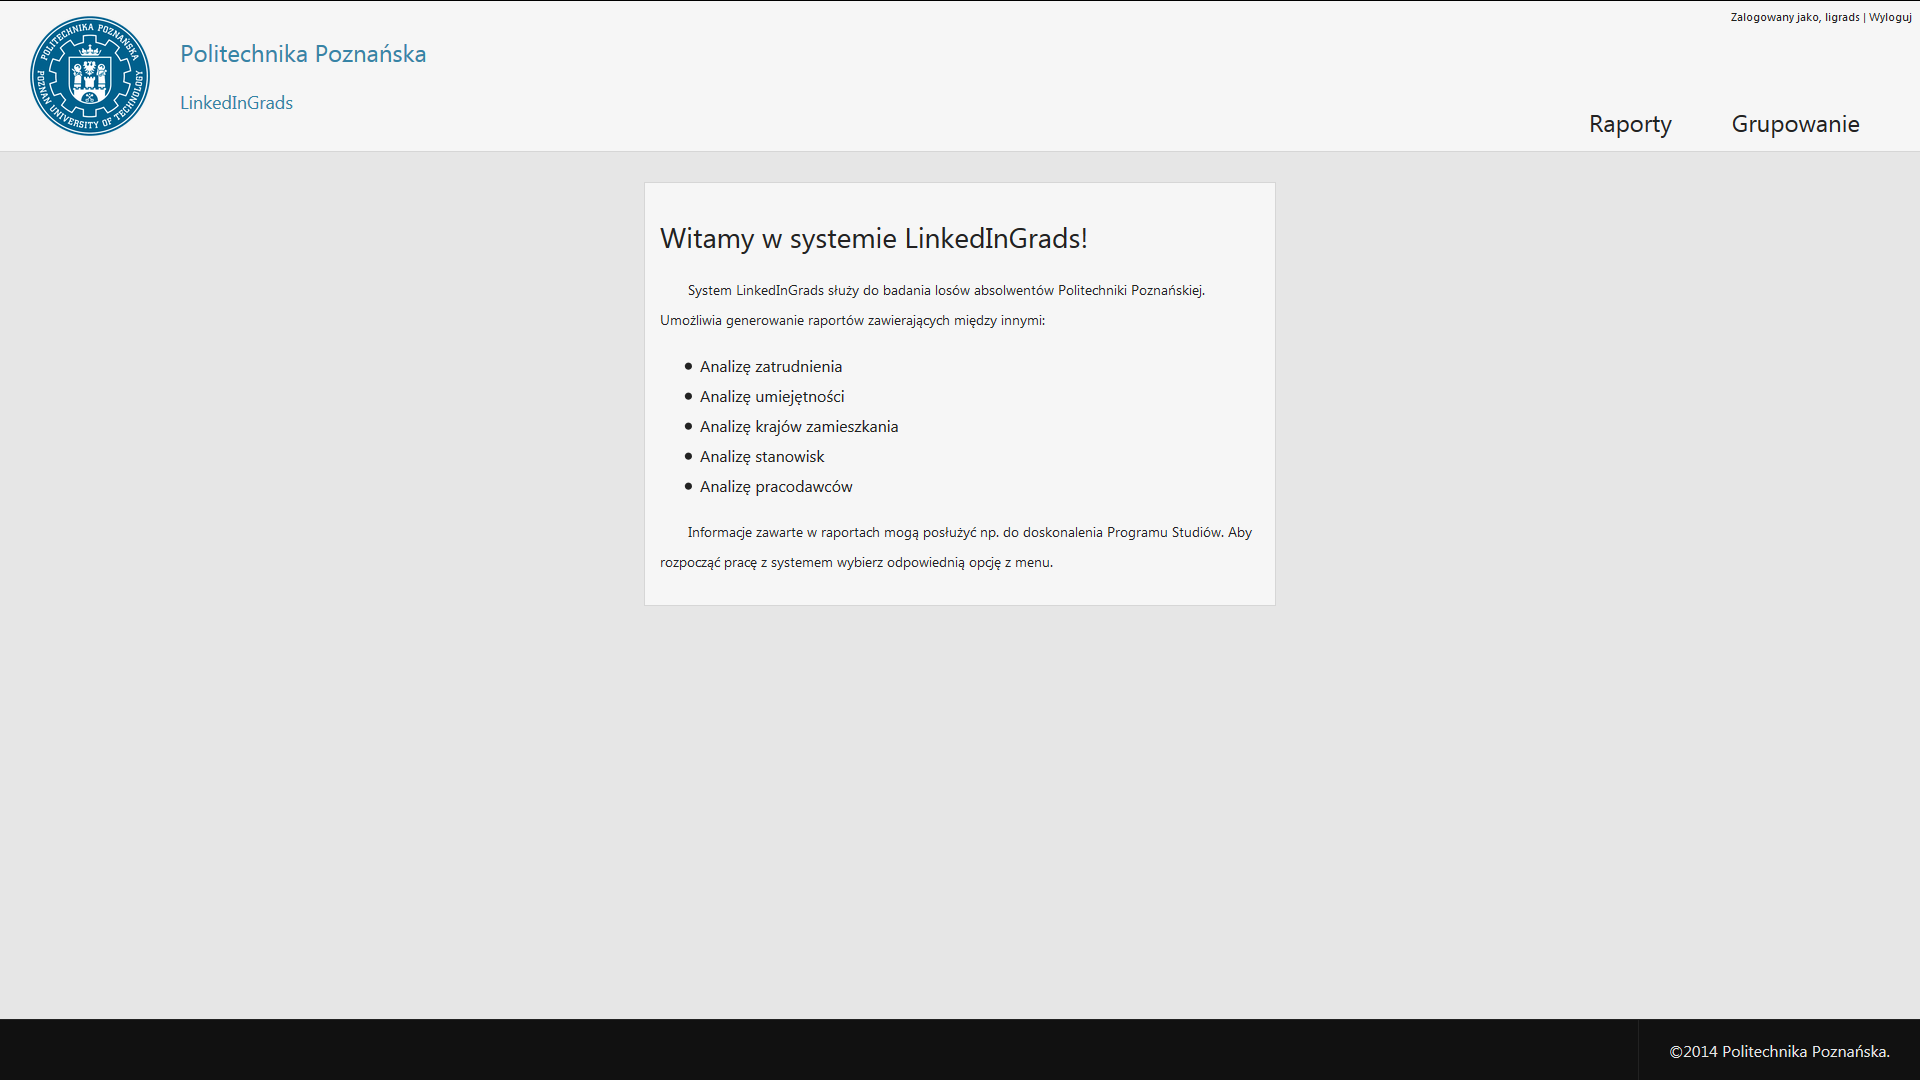
\includegraphics[width=15cm]{figures/image14}
\caption{Strona główna systemu LinkedInGrads}\label{rys:use-case-diagram}
\end{figure}

\begin{figure}[H] 
\centering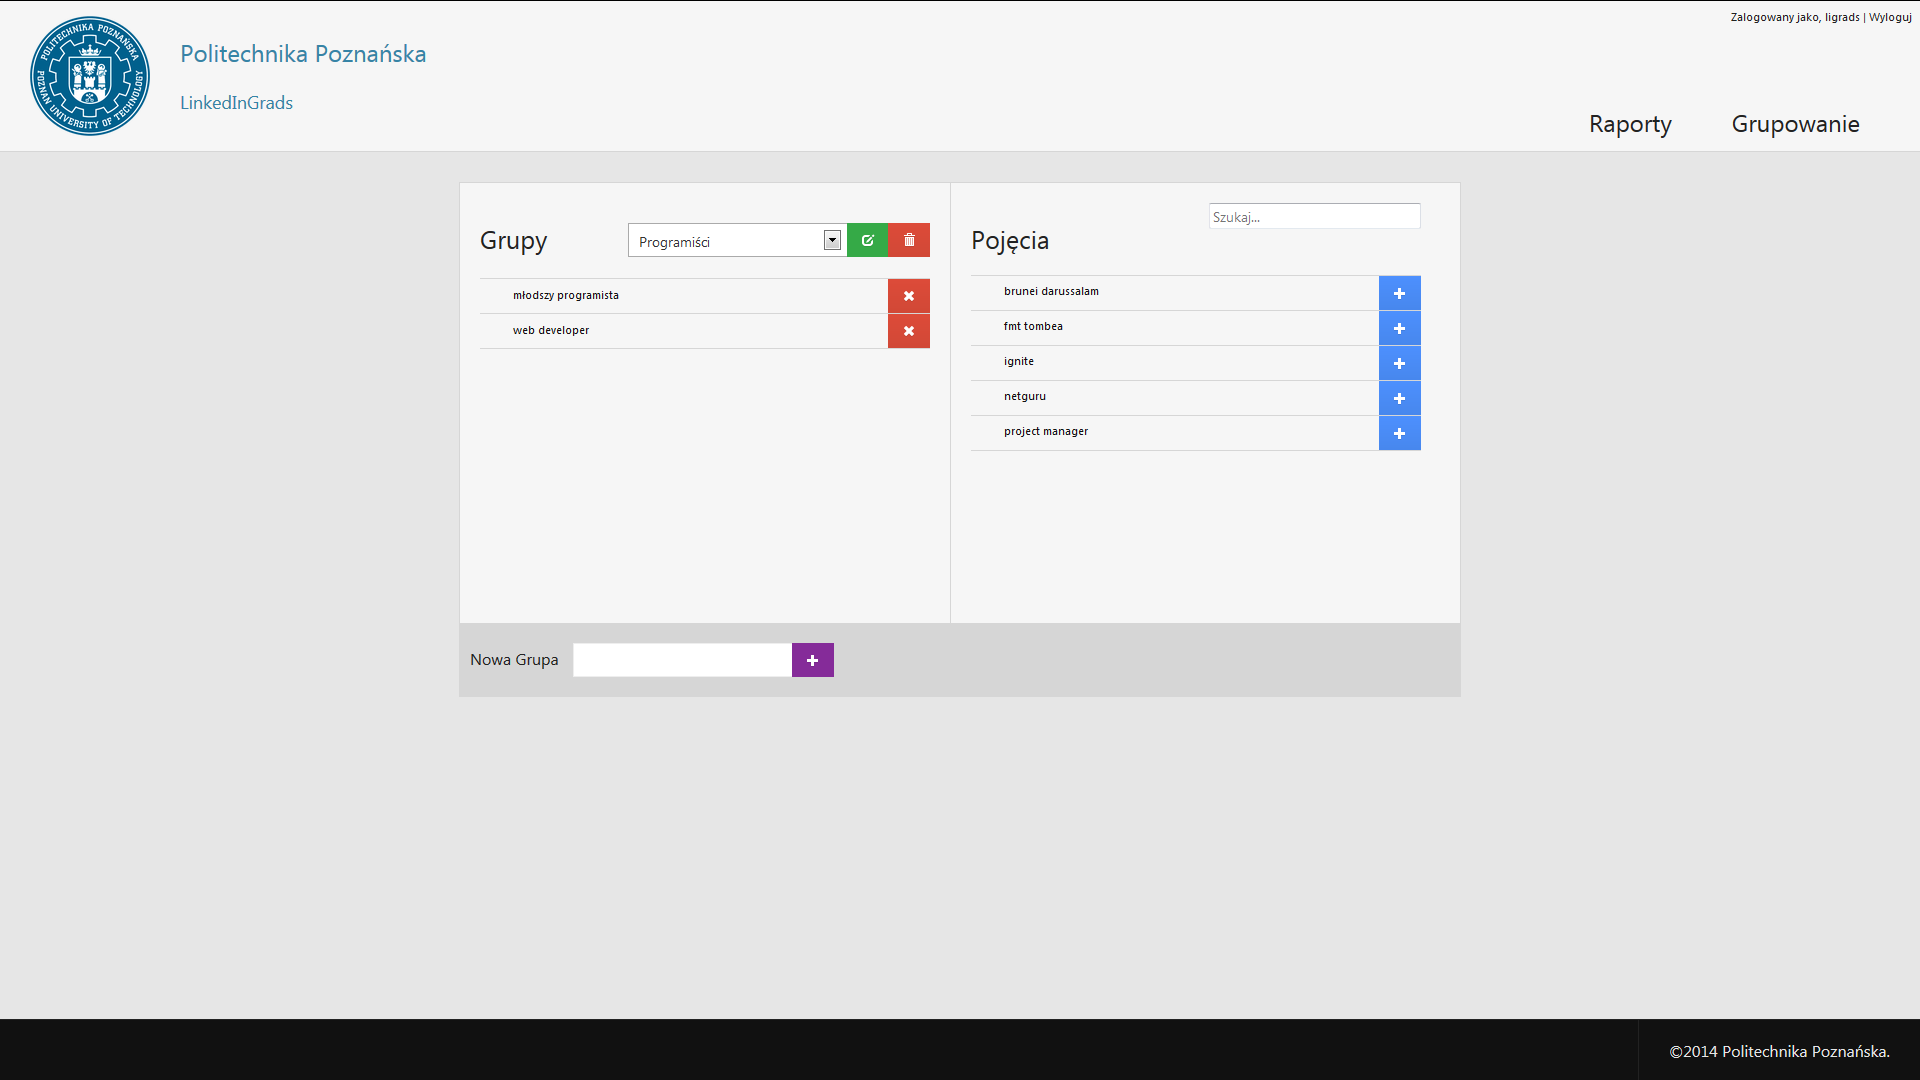
\includegraphics[width=15cm]{figures/image15}
\caption{Grupowanie pojęć}\label{rys:use-case-diagram}
\end{figure}

\begin{figure}[H] 
\centering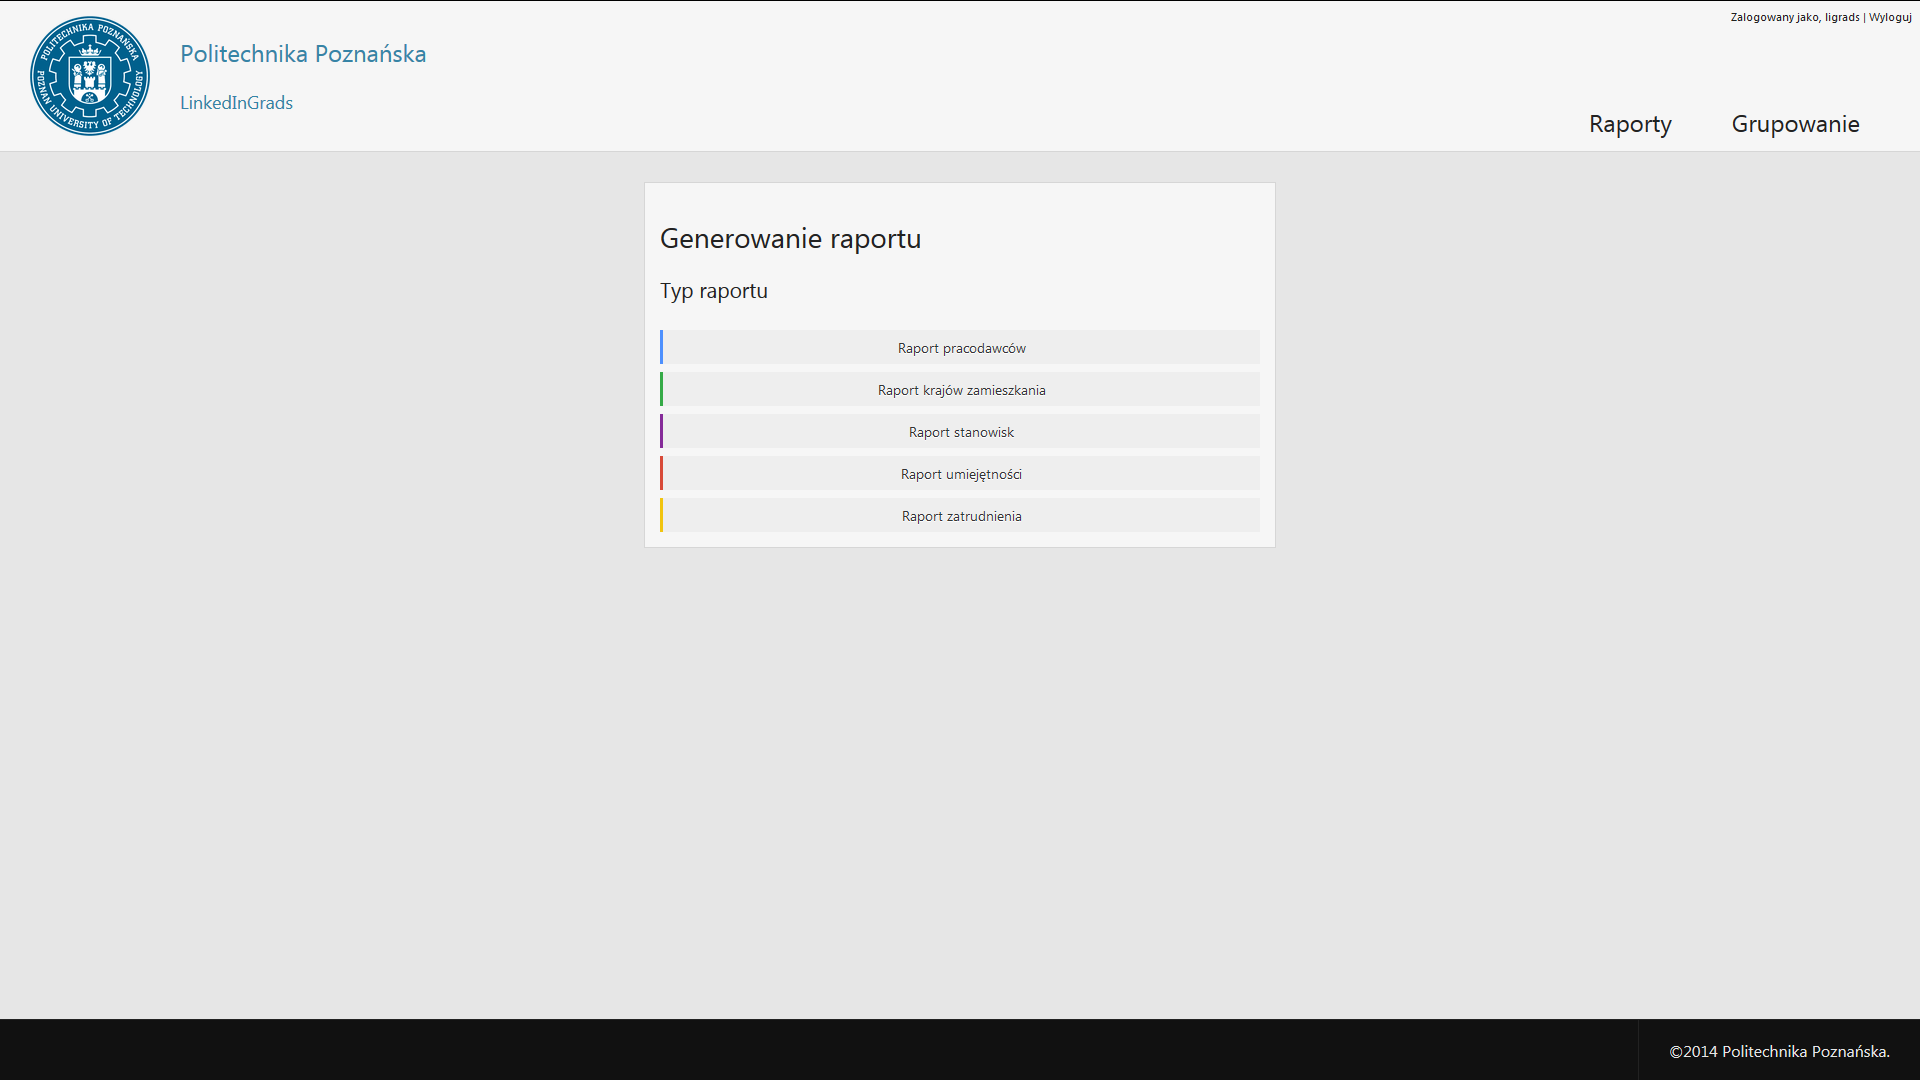
\includegraphics[width=15cm]{figures/image16}
\caption{Generowanie raportów - wybór dostępnego raportu}\label{rys:use-case-diagram}
\end{figure}

\begin{figure}[H] 
\centering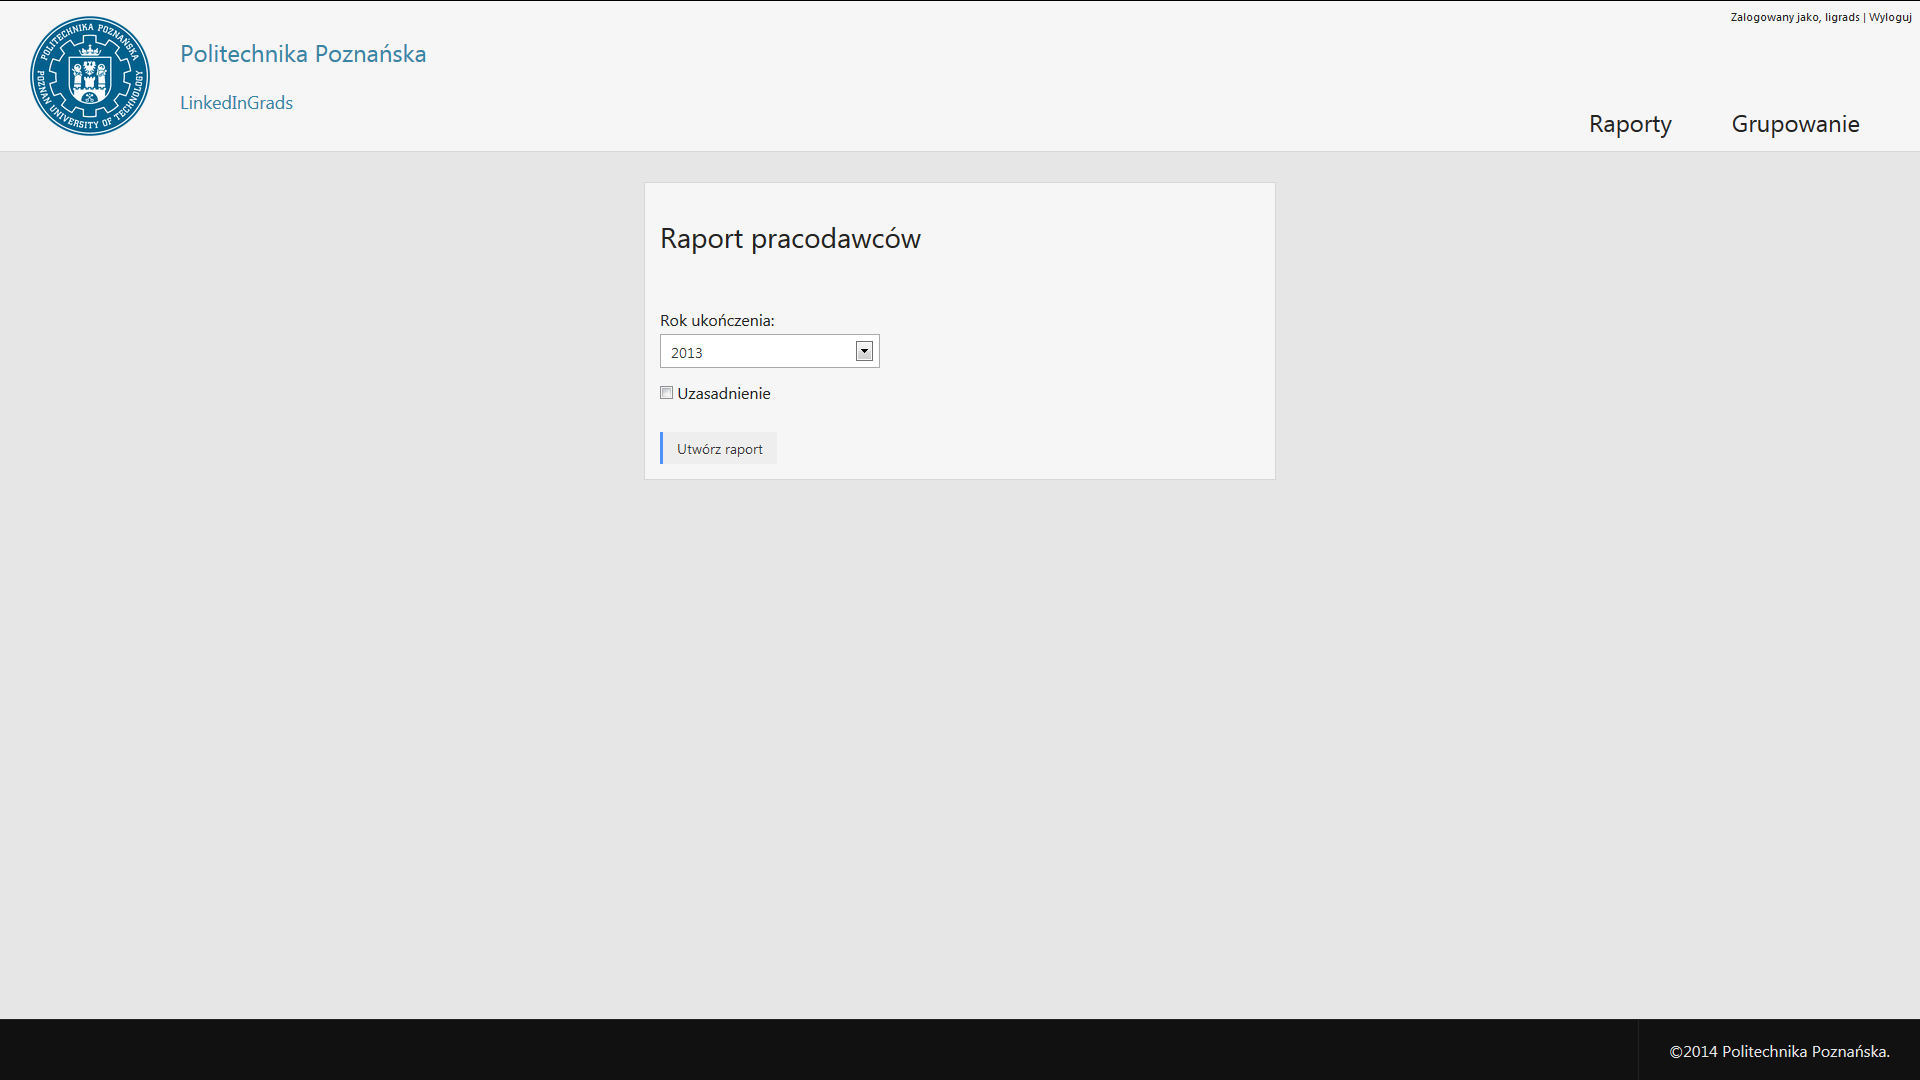
\includegraphics[width=15cm]{figures/image17}
\caption{Filtrowanie danych raportu}\label{rys:use-case-diagram}
\end{figure}

\begin{figure}[H] 
\centering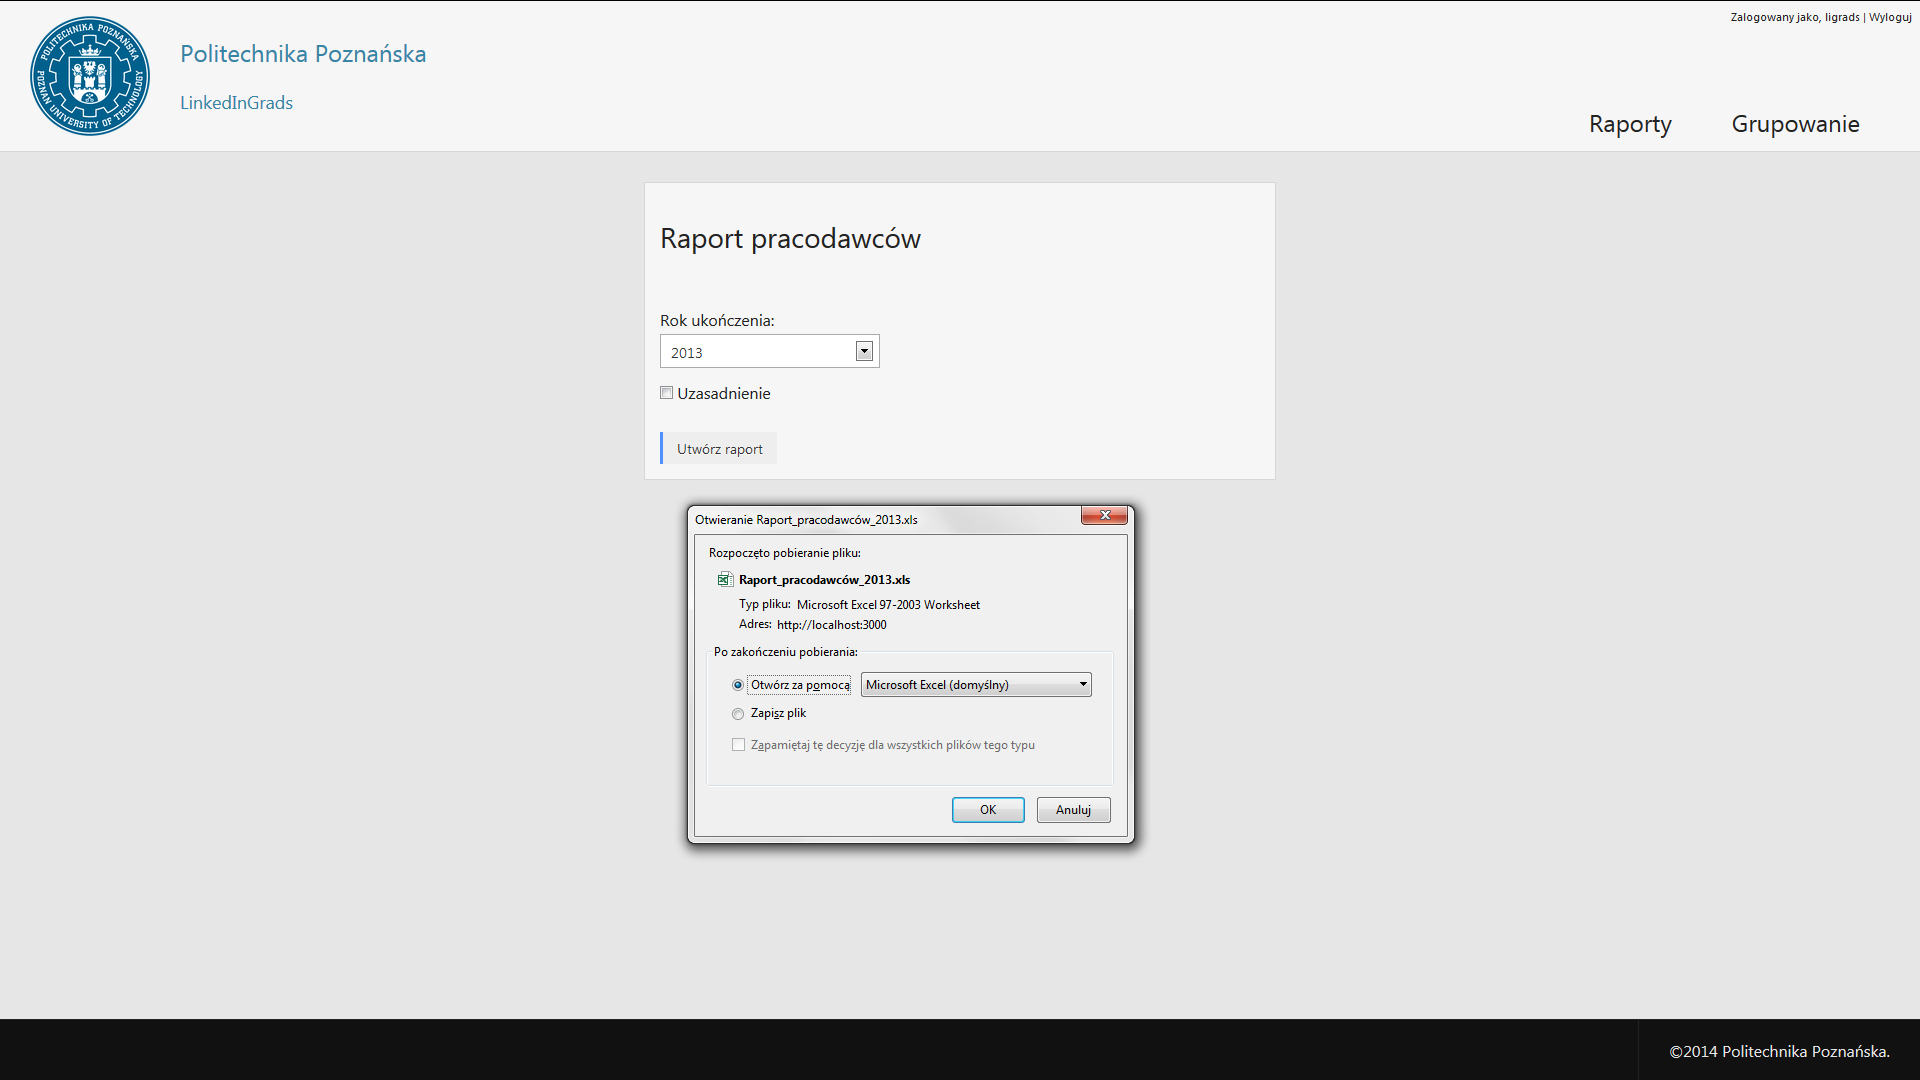
\includegraphics[width=15cm]{figures/image18}
\caption{Pobieranie gotowego raportu}\label{rys:use-case-diagram}
\end{figure}

\chapter{Schemat bazy danych}
\label{Chapterc1}

Dodatek opcjonalny, tutaj można zamieścić schematy bazy danych, jeśli nie zmieścił się w rozdziale o architekturze. Może być też tak, że będziecie mieli legen-czekaj-darny schemat o formacie A3 i będziecie go osobno drukować i wklejać w tym miejscu. Jeżeli nie chcecie tego dodatku, zakomentujecie załączenie tego pliku w \texttt{thesis-bachelor-polski.tex}.

\chapter{Literatura}

\begin{enumerate}
\item Nowelizacja Ustawy Prawo o szkolnictwie wyższym z dnia 18 marca 2012 r.
\item Rozporządzenie Ministra Nauki i Szkolnictwa Wyższego z dnia 29 września 2011 r. w sprawie warunków oceny programowej i oceny instytucjonalnej.
\item ISO/IEC FDIS 25010, Systems and software engineering – Systems and software Quality Requirements and Evaluation (SQuaRE) – System and software quality models, 2010.
\item Batsov B. The Ruby Style Guide. [on-line] https://github.com/bbatsov/ruby-style-guide. Dostęp 30.01.2014.
\end{enumerate}



% Bibliography (books, articles) starts here.
%%\bibliographystyle{plunsrt}{\raggedright\sloppy\small\bibliography{bibliography}}

% Colophon is a place where you should let others know about copyrights etc.
\ppcolophon

\end{document}
